%%%%%%%%%%%%%%%%%%%%%%%%%%%%%%%%%%%%%%%%%%%%%%%%%%%%%%%%%%%%%%%%%%%%%%%%%%%%%%%%
% 2345678901234567890123456789012345678901234567890123456789012345678901234567890
% 1         2         3         4         5         6         7         8

\documentclass[letterpaper, 10 pt, conference]{conf/ieeeconf}  % Comment this line out
% if you need a4paper
% \documentclass[a4paper, 10pt, conference]{ieeeconf}      % Use this line for a4
% paper

\IEEEoverridecommandlockouts                              % This command is only
% needed if you want to
% use the \thanks command
\overrideIEEEmargins
% See the \addtolength command later in the file to balance the column lengths
% on the last page of the document


% The following packages can be found on http:\\www.ctan.org
\usepackage{graphicx} % for pdf, bitmapped graphics files
\usepackage[table]{xcolor}
\usepackage{epsfig} % for postscript graphics files
\usepackage{mathptmx} % assumes new font selection scheme installed
\usepackage{times} % assumes new font selection scheme installed
\usepackage{amsmath} % assumes amsmath package installed
\usepackage{amssymb}  % assumes amsmath package installed
\usepackage{siunitx}
\usepackage{float}
\usepackage{pgf}
\usepackage{tikz}
\usetikzlibrary{arrows,automata,positioning}
\usepackage{hyperref}
\graphicspath{{./figures/}}
\usepackage{booktabs}
\usepackage{multirow}
\usepackage{pifont}% http://ctan.org/pkg/pifont
\usepackage{subcaption}
\newcommand{\cmark}{\ding{51}}%
\newcommand{\xmark}{\ding{55}}%
\usepackage{lipsum}
\setlength{\abovecaptionskip}{4pt}
\setlength{\belowcaptionskip}{-6pt}

\title{\LARGE \bf
  Autonomous Systems Practical Extension -- WBAI14001.2018-2019.2B \\
  Robotics Grasping
}

\author{Group: \texttt{grasp1} --- J\"{o}rdis Hollander (s2956543)}
% \thanks{The authors are with Faculty of Science and Engineering,
% University of Gronignen, The Netherlands.
% {\tt\small \{email1,email2\}@student.rug.nl}}
% }
\begin{document}

\maketitle
\thispagestyle{empty}
\pagestyle{empty}


%%%%%%%%%%%%%%%%%%%%%%%%%%%%%%%%%%%%%%%%%%%%%%%%%%%%%%%%%%%%%%%%%%%%%%%%%%%%%%%%
\begin{abstract}
  In this paper, automation via robotic arms is explored. A pipeline was developed
  to allow the Kinova MICO robot arm to grasp box objects from a table. There
  are several steps in this process.

  First, the position of the box object was detected. This was facilitated
  through provided code and leveraged the Robot Operating System ecosystem.
  Next, the angle of the box object was classified. The classifier was based on
  the Support Vector Machine learning model and was trained on a data-set of
  images of boxes in the real-world environment. Various preprocessing techniques
  and features were compared and contrasted in the development of the final
  classifier.
  Finally, the object was grasped. This was done using the data determined via
  the position detection and the angle classification. This data was then used to
  prepare a grasp which was then communicated to the MICO robot arm.

  The primary point of research is the comparison of the accuracy of the various
  classification methods. The pipelines for each classifier consisted of a
  preprocessing step and a feature extraction step.
  Various preprocessing steps and feature extraction steps were considered. The
  classification pipelines were tested for the product of the set of preprocessing
  steps and the set of feature extraction steps, in other words each preprocessing
  step was tested in conjunct with each feature extraction step. Each classifier
  was trialed in the simulation and tested on the real-world image data-set.

  The most-accurate classification pipeline was the pipeline which consisted of
  grayscaling the image as the preprocessing step and extracting the Histogram of
  Oriented Gradients as the feature extraction step. On the testing data-set
  (consisting of single boxes at various angles) this pipeline operated at 88.5\%
  accuracy.
\end{abstract}



%%%%%%%%%%%%%%%%%%%%%%%%%%%%%%%%%%%%%%%%%%%%%%%%%%%%%%%%%%%%%%%%%%%%%%%%%%%%%%%%
\section{Introduction}
% \noindent {\bf [2 points]}

Automation is a fundamental goal for AI and robotics. Through automation we
reduce unpleasant workloads for people, thereby freeing human capital to explore
other ventures, while simultaneously improving the accuracy and consistency of
repetitive tasks. This project explores automation by developing a pipeline that
allows a robot arm to grasp a box object from a table. This requires
identification of the position of the box, determination of the angle that the
box rests at (relative to the head of the arm), and communication of this
information to the arm so that a grasp attempt can be made.

The MICO arm is mounted to a table. A camera with a depth sensor is pointed at
the table with a fixed viewpoint providing context as to what is on the table.
Information from this camera is used to determine the positions of the objects
on the table as well as their angular orientation.

The positions of the boxes were identified through provided code that interacted
with ROS (Robot Operating System). This means that the focus of this project was
on classifying the angle of the box and on communicating this information to the
MICO arm. Classification entailed the creation of a classifier. To this end data
was collected in the form of images of various boxes at various angles. These
images were categorized manually into \textit{buckets} of different angles .
Support Vector Machines (SVM) are well suited to creating this sort of
multi-class classifiers \cite{Hsu2015}. However, building the classifier
requires extracting features from the images to train the statistical model. To
determine a robust solution a variety of prepocessing steps and extraction
techniques were attempted on the image data-set.

With the classifier in-place, the next stage is to implement the grasp
through message communication. With this the robot is ready to
grasp a box from the environment.

A description of the steps that must occur within the system are as follows:
\begin{enumerate}
\item The arm should return to its (predetermined) starting position.
\item The information on the positions of the objects that are visible to the
  camera are retrieved by querying the provided interface to the object detection
  server.
\item For each detected object, the image of the scene is fed into the
  classifier to determine the angle of the object.
\item Using the position of the object and the angle, the grasp is constructed
  and then relayed to the MICO arm.
\item For each object:
  \begin{enumerate}
  \item The arm moves above the object.
  \item The arm performs the grasp on the object.
  \item If the grasp is successful the arm moves the object to the
    (predetermined) ending position and releases the object.
  \end{enumerate}
\end{enumerate}

In section \ref{sec:method} the method for angle classification and object
communication are elaborated upon. In section \ref{sec:experiments} the
experimental setup and methodology is described, both of the simulation and of
the real-world composition. Section \ref{sec:results} details the experiments
that were undertaken and lists their results. Section \ref{sec:discussion}
discusses the results and forms a final conclusion. In this final section,
issues that arose throughout the development of the pipeline are also discussed.

% This section should introduce:
% \begin{itemize}
% \item the research topic(s) on the specific project you worked on (add references to at least one scientific paper, not weblinks)
% \item the main contribution of the work done: describe what your robot is suppose to do
% \item the outline of the rest of the report
% \end{itemize}



%%%%%%%%%%%%%%%%%%%%%%%%%%%%%%%%%%%%%%%%%%%%%%%%%%%%%%%%%%%%%%%%%%%%%%%%%%%%%%%%
\section{Method}
\label{sec:method}

% \noindent {\bf [4 points]}
% This section should describe the overall approach used in the work. The
% description can be subdivided in subsections to enhance readability. We added
% four subsections but you are free to add more.

The approach for developing the pipeline to allow the MICO arm to grasp a box
from a table consists of three main sections. A data-set of box images, a
classifier that determines the angles of the boxes, and a grasping function that
picks up and removes boxes from the table.

\subsection{Data-set Creation} %[1 point]
% Describe how you developed the part 1 of method. Do not write in terms of how
% you used the software tools, but write in terms of how you developed the part 1
% of the method.

The intention of the classifier is to determine the correct angle of orientation
of the box with respect to the arm. A data-set is needed to train this angle
classifier. As the context for the objects in the environment come from a
consistent fixed viewpoint camera, acquiring the requisite data is simple.

The provided object detection script captured the images from the environment.
These images were saved to disk and formed the basis of the data-set. 12 boxes
of a variety of shapes, sizes, and colors were used to create the data-set. Each
box was placed in up to 13 orientations and tagged with the angle their
orientation most closely corresponded to. The angles were one of \ang{0}.
\ang{45}, \ang{90}, and \ang{135}.

Previously, fewer types of boxes and a greater variety of possible angle values
were considered. However, this lead to inaccuracies in the resulting classifier.
These inaccuracies were resolved in two ways. By increasing the variety of boxes
in the data-set and by reducing the number of angles considered. This is
reasonable for this use-case as it was determined that the arm could grasp a
majority of the boxes in their various orientations with an angle of one of
\ang{0}, \ang{45}, \ang{90}, or \ang{135}.

\subsection{Constructing the Classifier} %[1 point]
With the data-set in place, the classifier could be constructed. The underlying
model for the classifier is a SVM. First, the data-set was partitioned into a
training set and a testing set.

Each image in the data-set underwent a form of preprocessing and feature
extraction prior to training (or indeed is also required before actual
classification). There were a variety of possible preprocessing steps and
feature extraction possibilities.

The preprocessing steps that were tested are as follows:
\begin{itemize}
\item Doing nothing to the image.
\item Converting the image to grayscale.
\item Blurring the image.
\item Blurring the grayscale version of the image.
\item Finding the contours of the image.
\item Finding the contours of the grayscale image.
\end{itemize}

Image blurring and contour detection are performed via image filters
(convolution kernels) and were executed using \texttt{ImageFilter.BLUR} and
\texttt{ImageFilter.CONTOUR} which are built-in to the Python \texttt{Pillow}
library. For reference, the convolution kernel for blurring may be seen in
equation \eqref{eq:blur} and the convolution kernel for contour detection may be
seen in equation \eqref{eq:contour}.

\noindent\begin{minipage}{.5\linewidth}
  \begin{equation}
    \begin{bmatrix}
      1 & 1 & 1 & 1 & 1\\
      1 & 0 & 0 & 0 & 1\\
      1 & 0 & 0 & 0 & 1\\
      1 & 0 & 0 & 0 & 1\\
      1 & 1 & 1 & 1 & 1\\
    \end{bmatrix}
    \label{eq:blur}
  \end{equation}
\end{minipage}%
\begin{minipage}{.5\linewidth}
  \begin{equation}
    \begin{bmatrix}
      -1 & -1 & -1\\
      -1 &  8 & -1\\
      -1 & -1 & -1\\
    \end{bmatrix}\\
    \label{eq:contour}
  \end{equation}
\end{minipage}\\

Next, the feature extraction steps must be considered. According to Dong et al.,
features based on a Histogram of Oriented Gradients (HOG) and Scale Invariant
Feature Transform (SIFT) are two widely-used techniques with good performance
for object recognition \cite{Dong2010}.

The HOG features are computed through several steps \cite{Dalal2005}. First, the
input image undergoes gamma normalization, whereby square-root gamma compression
is applied across each color channel. This reduces the influence of illumination
in the final feature vector. Next, the gradient image is computed along the $x$
and $y$ of the image. For color images, this is computed across each channel,
with the resulting gradient vector corresponding to the gradient vector of the
largest norm for that pixel across each channel. The next step is orientation
binning. The image is split into cells, each of which consist of $16 \times 16$
pixels. Each cell accumulates the information of the orientation of the
gradients contained within it. This information is then used to divide the
gradient angle into bins spaced over \ang{0} -- \ang{180}. These HOG descriptors
are then combined into the final feature vector.

As described by Lowe, the computation of SIFT features consists of four primary
steps \cite{Lowe2004}. The first step is scale-space extrema detection which
uses a difference-of-Gaussian function to determine points that are invariant to
scale and orientation. This is used to compute the difference between the input
image and a copy of the image that has been scaled. Each point in the resulting
difference is compared against neighboring points at the same scale and
neighboring points up and down the scale. If the point is a maximum or minimum
against these points then it is an extrema. The second step is keypoints
localization and involves identifying keypoints among the identified extrema. A
model is fit to determine location and scale and filters candidate keypoints
based on stability. The third step is orientation assignment and assigns
orientations to each keypoint based on local image gradient directions. This
provides invariance to image rotation. The magnitudes and orientations of the
local image gradients are sampled around each keypoint location. This gradient
information is rotated to align with the keypoint and weighted by a Gaussian
with variance proportional to the keypoint scale. This is then used to create
the keypoint descriptors is the form of histograms over a window in a keypoint.
This final step provides orientation invariance and resistance to local shape
distortion and changes in illumination.

However, the resulting keypoint descriptors are not suitable as a feature to
train the SVM due to the differing number of keypoints that may be extracted
from each image. This is resolved by computing a Visual Bag of Words representation
by using KMeans clustering on the extracted SIFT descriptors. The descriptor of
the image is then computed by assigning each SIFT of the image to one of the
K-clusters. The resulting histogram is then normalized with L1 normalization and
is now of consistent length. This is then used as the basis for the SVM.

These feature extraction techniques were contrasted against simply using the
entire preprocessed image as the feature. Thus, the feature extraction steps are
as follows:\\
\begin{itemize}
\item Leaving the preprocessed image as is (for comparison purposes).
\item Extracting HOG features.
\item Extracting SIFT features.
\end{itemize}

The combination of each preprocessing step and each feature extraction step
resulted in a variety of pipelines. The most accurate of these pipelines was
included in the final application.

\subsection{Grasping} %[1 point]
Grasping requires the position and angle for each object on the table. The
position is determined through provided code and the angle may be determined via
the classifier. These attributes for the object are then added to the internal
representation of the environment known as the octomap. With the objects in the
octomap, the provided code and the \textit{ROS} ecosystem can handle the motion
planning. As a result, grasping then consisted of setting the starting state,
moving the arm to the position above the object, and orienting the arm to match
the angle of the object. The object is then grasped, with the arm then moving to
a predetermined final position. If all the potential grasps fail, the arm then
returns to the starting position. The messages for communicating with the arm
were constructed using the \textit{MoveIt} framework with the path planning and
inverse kinematics integrated into the \textit{ROS} ecosystem facilitating the
actual motion computation.

\subsection{Behavior/Architecture} %  [1 points]
% Insert here a figure representing the state machine designed for the overall
% system. Describe the different states/nodes, explain and show the overall system
% behavior. Explain the design choices of your behaviour system (i.e., why did you
% create a sub-behaviour/node for that specific task?). Make sure your state
% machine is readable.
To describe the overall behavior of the system it is useful to consult a state
machine describing the basic states of the system during execution. See figure \ref{fig:1}.

\begin{figure}[H]
  \centering
  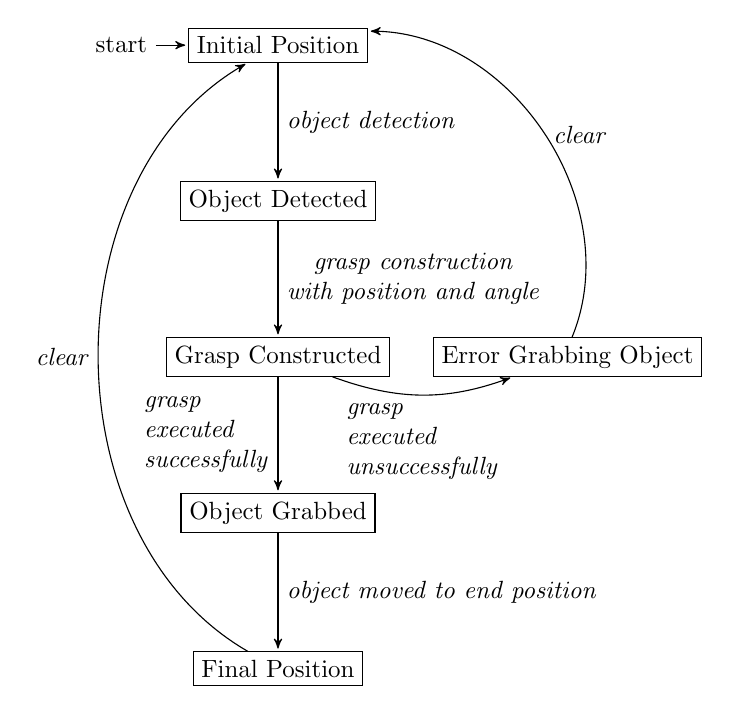
\begin{tikzpicture}[->,>=stealth', shorten >=1pt, auto,
    node distance=2.2cm, scale=0.9,
    transform shape, align=center,
    state/.style={rectangle, draw}
    ]

    \node[initial,state] (A)                {Initial Position};
    \node[state]         (B) [below of=A]   {Object Detected};
    \node[state]         (C) [below of=B]   {Grasp Constructed};
    \node[state]         (D) [below of=C]   {Object Grabbed};
    \node[state]         (E) [right=0.6 of C] {Error Grabbing Object};
    \node[state]         (F) [below of=D]   {Final Position};

    \path
    (A) edge node                                    {\textit{object detection}}                    (B)
    (B) edge node                                    {\textit{grasp construction}\\ \textit{with position and angle}} (C)
    (C) edge node[align=left, left]                  {\textit{grasp}\\ \textit{executed}\\ \textit{successfully}}               (D)
    (C) edge [bend right=20] node[align=left, below] {\textit{grasp}\\ \textit{executed}\\ \textit{unsuccessfully}}             (E)
    (D) edge node                                    {\textit{object moved to end position}}                 (F)
    (F) edge [bend left=60] node                     {\textit{clear}}                                        (A)
    (E) edge [bend right=56] node[right]             {\textit{clear}}                                        (A);
  \end{tikzpicture}
  \caption{\label{fig:1}State Machine for Overall System}
\end{figure}
The starting state for the system is with the arm being in its \textbf{Initial
  Position}. This entails the arm moving to a predefined start position with its
fingers being in the open grasp position. Upon the detection of an object we
shift to the \textbf{Object Detected} state. As the object has been detected its
position may be extracted by communicating with the interface to the object
detection server. This also provides an image which may be run through the angle
classifier. This provides both the position and the angle which allows the
transition to the next state with the \textbf{Grasp Constructed}. A grasp may
fail or may be successful. On failure the system faced an \textbf{Error Grabbing
  Object} which is responded to by clearing the state and returning the arm to the
\textbf{Initial Position}. If the grasp has executed successfully the arm has
the \textbf{Object Grabbed}. In this state the arm moves to the \textbf{Final
  Position}, opening the fingers and releasing the object. Finally the arm then
returns to the \textbf{Initial Position}. This cycles continues while there are
objects to be detected.


%%%%%%%%%%%%%%%%%%%%%%%%%%%%%%%%%%%%%%%%%%%%%%%%%%%%%%%%%%%%%%%%%%%%%%%%%%%%%%%%
\section{Experiments}
\label{sec:experiments}
% \noindent {\bf [1.5 points]}
The experiments that could be undertaken fall into two categories. Experiments
testing the functionality of the system as a whole and experiments testing the
functionality of the sub-components of the system. Of the three primary
sub-components: object detection, angle classification, and grasping, angle
classification is of particular importance. As a result, the trials were focused
on testing the entire functionality of the system and of the capabilities of the
angle classifier specifically.

\subsection{Experimental setup}
The real-world setup consists of a table with the Kinova MICO arm mounted to it.
There is a stationary camera providing a fixed viewpoint of the table. Testing
the overall capabilities of the system consists of placing boxes onto the table
and running the program. If successful the arm will grasp each box and remove
them from the table, dropping them in a bin. An image of the environment may
be seen in figure \ref{fig:real_environment}.

\begin{figure}[H]
  \centering
  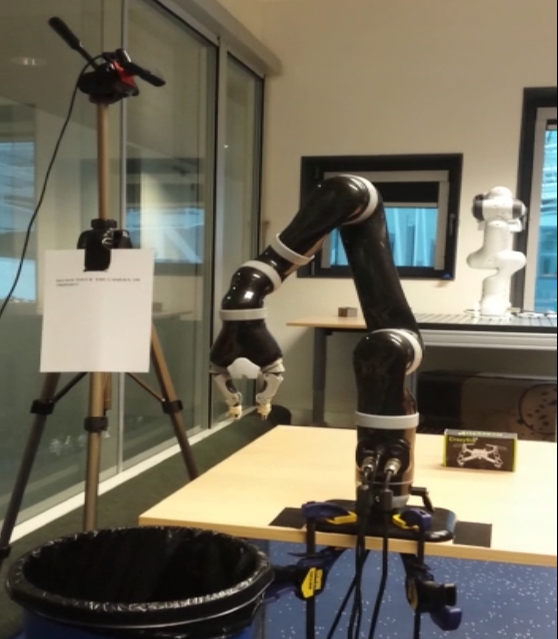
\includegraphics[width=0.8\linewidth]{real_environment.png}
  \caption{\label{fig:real_environment} Real-world Execution Environment}
\end{figure}

Aside from the real-world setup, the system was also developed and tested using
a simulation. \textit{RViz} and \textit{Gazebo} were the tools used to interact
and view this environment. As may be seen in figure
\ref{fig:virtual_environment}, the virtual environment also consisted of an arm
and a fixed viewpoint camera. This camera provides a snapshot of the scene
containing the target boxes. The success criterion for the simulation is also a
successful grasp of the boxes in the simulated environment.

\begin{figure}[H]
  \centering
  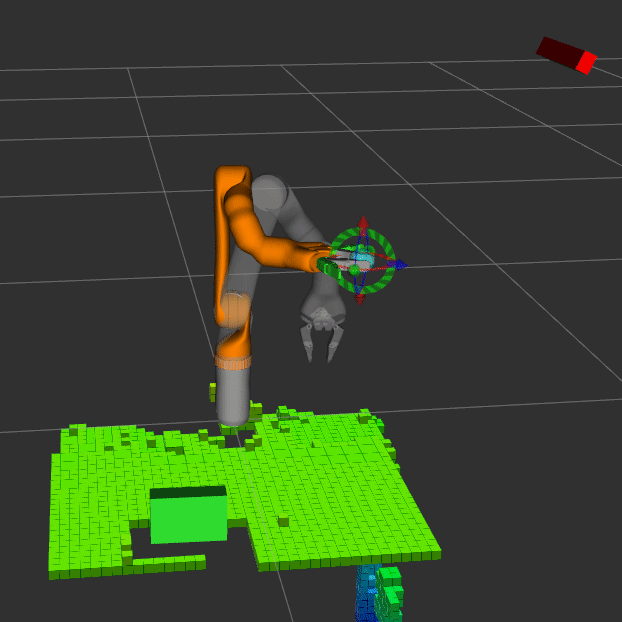
\includegraphics[width=0.8\linewidth]{virtual_environment.png}
  \caption{\label{fig:virtual_environment} Visualization of Virtual Environment}
\end{figure}

\subsection{Experiments on the Classifiers}
With respect to testing the classifiers, the setup consisted of constructing the
various classification pipelines and executing them on the testing data-set. The
value measured was on the accuracy of the classifier and was computed as
follows:
\begin{equation*}
  \text{accuracy} = \dfrac{\text{number of images classified correctly}}{\text{total number of images}}
\end{equation*}

The testing data-set consisted of 85 images of boxes on the table positioned in
angles from \ang{0} to \ang{180}. For each image the system should classify it
as the angle it is closest to out of \ang{0}, \ang{45}, \ang{90}, and \ang{135}.
The results for the various pipelines are presented in section
\ref{sec:results}. 85 images provides a reasonably large data-set for testing
and exhausts the boxes of the right dimensions and mass that were reasonably
accessible.

The most successful pipeline from these tests, i.e. grayscale preprocessing with
HOG feature extraction, was used as the pipeline for the experiments on the
overall system.

\subsection{Experiments on the Overall System}
For testing the overall system, three categories were candidates for
measurement: the execution time, the accuracy of the system, and the robustness
of the system.
\subsubsection{Testing Timing}
How long does it take to remove one box from a table? Measuring this consisted
of setting up a trial box in the environment and executing the system. The time
taken from the start of the execution to the end (with the arm returning to the
start position) was measured. Though the execution time was not the priority for
the project, it was important to ensure that the real world execution time was
reasonable.

\subsubsection{Testing Accuracy of Single Box Configurations}
For the real-world environment, 7 different boxes were tested in 4 different
configurations each. The boxes may be seen in the appendix. Each test for each
box for each configuration was trialed twice. This resulted in a total of 56
trials. The four configurations were \ang{0}, \ang{45}, \ang{90}, and \ang{135}.

For the simulated environment, the same trials were conducted. Boxes of similar
proportions were tested with the four configurations of \ang{0}, \ang{45},
\ang{90}, and \ang{135}. As may be seen in the results for these trials, the
system was very inaccurate in the simulation. As a prerequisite for the
robustness trails the system should perform well in the single box configuration
test. Thus, the trials for robustness were not conducted for the simulation.

\subsubsection{Testing Robustness}
The robustness of the system was tested qualitatively. A variety of edge cases
and multiple box configurations were tested. Each configuration was trialed
twice. The results include a list of the various configurations and whether the
system functioned correctly for that configuration. The limits that were tested
are as follows:

\begin{itemize}
\item \textbf{Limits of possible locations to grasp on the table.}
  There are two obvious limiting factors. First, the box must be within the
  bounds of the octomap virtual planning environment. Second, the box must be
  reachable by the arm. Problem cases are when the box is too far away from the
  arm or too close for the joints of the arm to contort themselves. The limits are
  defined in terms of the distance in \si{\centi\meter} from the base of the arm.
  These limits will be tested with box 1 from figure \ref{fig:test_boxes} as it
  is easy to detect, classify, and grasp.
\item \textbf{Limits of object detection (minimum size and transparency).}
  As may be seen in figure \ref{fig:1}, \texttt{object detection} is required
  before any other step in the main execution pipeline. Obviously, the object must
  be within the visual field of the camera. However, there may be a lower limit on
  dimensions of the object where it stops being detected. The system was tested on
  boxes of different sizes to determine this lower limit. The system was also
  tested on transparent objects to determine if transparency would cause issues in
  object detection.
\item \textbf{Limits of grasping (object thickness, object height):}
  When grasping an object the system is conservative in how far the fingers
  close. This is to prevent the arm from crushing the objects that it is grasping.
  Additionally, the arm may be unable to grasp an object which is too short. These
  limits were tested on boxes of different thicknesses and heights to determine
  possible limitations.
\item \textbf{Limits of classification (various object dimensions).}
  Boxes were acquired outside of the initial testing data-set to test edge cases
  in object classification. This included boxes, that were tall and
  thin or short and fat.
\item \textbf{Limits of classification with multiple independent objects.}
  The images the classifier was trained on consisted of single boxes. Multiple
  boxes being present in a scene may cause issues in angle classification. This
  was tested by placing multiple boxes in the scene simultaneously to determine
  how the classifier would react. Some tests involved placing boxes behind each
  other and in other tests the boxes were separated with space between each other.
\item \textbf{Limits of classification with stacked objects.}
  As with the previous limitation, stacked objects may pose a problem. The
  configurations that were considered were boxes that were stacked with the same
  orientation and perpendicular to each other. Boxes of different sizes that were
  stacked were also considered in the same fashion.
\end{itemize}

The aim of these tests was to provide a sense of the operational boundaries of
the system and to help guide future development.
The specific tests and their outcomes are detailed in section \ref{sec:results}.
\vspace{-0.6em}
% This section should present the experimental setup and should to show that your
% system is working correctly. You need to come up with a way to show that your
% system is working correctly. It is recommended that you show the working of the
% complete system with one experimental setup, only if your system isn't 100\%
% working you can show each sub-system individually (this means a lot more work
% though), or if you think it is important to show the performance of a
% sub-system. Also run the experiments in simulation (if possible in your
% project), in order to make a comparison with the real world and simulation.
% Think about how many trials you want to perform, you need to explain why you
% picked that number of trials. You need to determine what you are measuring
% (which can be multiple things), e.g., accuracy, robustness, timing.

% In short, this section should:
% \begin{itemize}
% \item Contain a description of the experimental set-up
% \item Present the trials (in simulation and/or on the real robot)
% \item Show that the overall system works, if not each sub-part should be tested.
% \end{itemize}

\section{Results}
\label{sec:results}
% \noindent {\bf [1.5 points]}
% This section should present your results. Present your results in tables/graphs and write about what these results mean in detail.

\subsection{Results for the Timing Experiments}
For the real world environment the runtime was approximately 44 seconds with a
variance of approximately 3 seconds based on the position of the box on the
table. The results for these tests in the virtual environment were highly
variable due to limitations of the simulation. It is of little real world
significance and depends highly on the computational resources available. These
experiments have confirmed that the real world execution time is reasonable.

\subsection{Results for Classifier Experiments}
The classifier pipelines consist of a preprocessing technique and a feature
extraction technique. In table \ref{tab:classification} the accuracy for each
pipeline (preprocessing technique $\times$ feature extraction) is shown.
\begin{table}[h]
  \centering
  \begin{tabular}{l c c c}
    \toprule
    \multirow{2}{*}[-0.5\dimexpr \aboverulesep + \belowrulesep + \cmidrulewidth]{Preprocessing Technique} & \multicolumn{3}{c}{Feature Extraction}\\
    \cmidrule(lr){2-4}
                                                                                                          & Raw Image & HOG & SIFT \\
    \midrule
    Color (no preprocessing)     & 75.6\% & 73.5\%                    & -- \\
    Contour extraction           & 62.9\% & 70.1\%                    & -- \\
    Blur                         & 75.6\% & 87.3\%                    & -- \\
    Grayscale                    & 73.4\% & \cellcolor{blue!25}88.5\% & 76.6\% \\
    Grayscale contour extraction & 62.9\% & 84.2\%                    & 73.4\% \\
    Grayscale blur               & 76.6\% & 88.4\%                    & 77.8\% \\
    \bottomrule
  \end{tabular}
  \caption{Accuracy of Various Classification Pipelines}
  \label{tab:classification}
\end{table}

First, it is interesting to note how high the accuracy is for the pipeline
constructed from unprocessed raw images. However, this is likely to hold only
for the limited scope of the project. As more complex boxes or orientations
enter the fray it is unlikely for this pipeline to maintain its accuracy.

In the case of HOG feature extraction it is notable that the pipelines with the
preprocessing techniques involving grayscaling operate at a higher accuracy. The
intuition for this is that the absence of color improves the consistency of HOG
feature extraction. The same logic lead to the incorporation of blurring.

Blurring the image (either in color or in grayscale) seems to result in a
relatively accurate classifier irrespective of the feature extraction technique
employed.

However, simply grayscaling the image and performing HOG feature
extraction operates the best at 88.5\% accuracy.

\subsection{Results for Overall System Accuracy Experiments}

Table \ref{tab:trials_real_world} show the results for the trials for the
various orientations for boxes 1--7 in the real-world environment. A \cmark~
indicates if the trial was successful (the box was grasped and removed from the
table), while a \xmark~ indicates if the trial was unsuccessful.
\begin{table}[H]
  \centering
  \begin{tabular}{c c c c c c c c c}
    \toprule
    \multirow{4}{*}[-0.5\dimexpr \aboverulesep + \belowrulesep + \cmidrulewidth]{Box} & \multicolumn{8}{c}{Orientations}\\
    \cmidrule(rl){2-9}
                                                                                      & \multicolumn{2}{c}{\ang{0}} & \multicolumn{2}{c}{\ang{45}} & \multicolumn{2}{c}{\ang{90}} & \multicolumn{2}{c}{\ang{135}} \\
    \cmidrule(lr{2pt}){2-3}
    \cmidrule(l{2pt}r{2pt}){4-5}
    \cmidrule(l{2pt}r{2pt}){6-7}
    \cmidrule(l{2pt}r{2pt}){8-9}
                                                                                      & 1      & 2      & 1      & 2      &  1     & 2      &  1     &  2     \\
    \midrule
    1 & \cmark & \cmark & \cmark & \cmark & \cmark & \cmark & \cmark & \cmark \\
    2 & \cmark & \cmark & \cmark & \cmark & \cmark & \cmark & \cmark & \cmark \\
    3 & \cmark & \cmark & \cmark & \cmark & \cmark & \cmark & \cmark & \cmark \\
    4 & \cmark & \cmark & \cmark & \cmark & \cmark & \cmark & \cmark & \cmark \\
    5 & \cmark & \cmark & \cmark & \cmark & \cmark & \cmark & \cmark & \cmark \\
    6 & \cmark & \cmark & \cmark & \cmark & \cmark & \cmark & \cmark & \cmark \\
    7 & \cmark & \cmark & \cmark & \cmark & \cmark & \cmark & \cmark & \cmark \\
    \bottomrule
  \end{tabular}
  \caption{Trials for System in Real-world Environment}
  \label{tab:trials_real_world}
\end{table}

As may be seen, the system was successful in every case. This may be explained
by the relative simplicity of these orientations. When running the classifier
based on grayscaled HOG features on the subset of the testing data-set that
correspond to these images, it operates at a 96\% accuracy. However, as may be
seen in table \ref{tab:trials_simulated} this does not hold when considering the
trials in the simulated environment.

\begin{table}[H]
  \centering
  \begin{tabular}{c c c c c c c c c}
    \toprule
    \multirow{4}{*}[-0.5\dimexpr \aboverulesep + \belowrulesep + \cmidrulewidth]{Box} & \multicolumn{8}{c}{Orientations}\\
    \cmidrule(rl){2-9}
                                                                                      & \multicolumn{2}{c}{\ang{0}} & \multicolumn{2}{c}{\ang{45}} & \multicolumn{2}{c}{\ang{90}} & \multicolumn{2}{c}{\ang{135}} \\
    \cmidrule(lr{2pt}){2-3}
    \cmidrule(l{2pt}r{2pt}){4-5}
    \cmidrule(l{2pt}r{2pt}){6-7}
    \cmidrule(l{2pt}r{2pt}){8-9}
                                                                                      & 1      & 2      & 1      & 2      &  1     & 2      &  1     &  2    \\
    \midrule
    1 & \cmark & \cmark & \xmark & \xmark & \cmark & \cmark & \xmark & \xmark \\
    2 & \cmark & \cmark & \xmark & \xmark & \cmark & \cmark & \xmark & \xmark \\
    3 & \cmark & \cmark & \xmark & \xmark & \cmark & \cmark & \xmark & \xmark \\
    4 & \cmark & \cmark & \xmark & \xmark & \cmark & \cmark & \xmark & \xmark \\
    5 & \cmark & \cmark & \xmark & \xmark & \cmark & \cmark & \xmark & \xmark \\
    6 & \cmark & \cmark & \xmark & \xmark & \cmark & \cmark & \xmark & \xmark \\
    7 & \cmark & \cmark & \xmark & \xmark & \cmark & \cmark & \xmark & \xmark \\
    \bottomrule
  \end{tabular}
  \caption{Trials for System in Simulated Environment}
  \label{tab:trials_simulated}
\end{table}

For the simulated environment every box that is at \ang{45} and \ang{135} fails.
As a result, the accuracy in the simulated environment is 50\%. The only portion
of the pipeline that could lead to this sort of failure for these simple cases
is the classifier. When testing this assumption, it was noted that each image
from the simulated environment corresponding with the angles of \ang{45} and
\ang{135} were classified as \ang{0} or \ang{90} degrees. The reasons for this
are elaborated on in section \ref{sec:discussion}.

Ultimately, irrespective of the issues in the simulation, the results for the
real-world execution holds the most significance. Thus, it is now
important to consider the real-world performance for more complex scenarios.

\subsection{Trials for Robustness of Overall System in Real-world Environment}
The trials for robustness are qualitative and used to determine the limits of
the system. So, a variety of limits associated with different parts of the
system were considered.

\subsubsection{Limits of possible locations to grasp on the table}
For the tested box which was \SI{9.5}{\centi\meter} high, it could be grasped
when it was a minimum of \SI{10}{\centi\meter} from the base of the arm and a
maximum at the very edge of the octomap at approximately \SI{67}{\centi\meter}
from the base of the arm. When it was placed closer or further away the arm was
unable to perform a successful grasp.

\subsubsection{Limits of object detection (minimum size and transparency)}
If the object is transparent, such as with the tested plastic bottle, the system
fails to detect the presence of the object. Additionally, when the system was
tested with a Rubix cube with each side being \SI{1.5}{\centi\meter}, it was
discovered that the system could only detect the object if it was sufficiently
close to the camera. When the cube was placed more than \SI{45}{\centi\meter}
away from the edge of the table facing the camera, it ceased to be detected.
Thus, it is clear that based on the size and proximity to the camera the ability
of the system to detect objects varies. The precise relationship and the lower
limits of this were not determined.

\subsubsection{Limits of grasping (object thickness, object height)}
During the tests on the various boxes it was determined that the minimum
thickness required for the object to be grabbed was approximately
\SI{1.3}{\centi\meter}. Any smaller and the grip was too weak to be able to grab
the object.

If the arm is oriented correctly, it is able to pick up objects only
\SI{1}{\centi\meter} high. This was tested on a small box (\SI{1}{\centi\meter}
x \SI{4}{\centi\meter} x \SI{6}{\centi\meter}). However, if the orientation
results in any of the fingers scraping against the table, the arm responds with
an internal error signaling the end of the grasp.

\subsubsection{Limits of classification (various object dimensions)}
When testing additional boxes outside of the original testing data-set, it was
determined that tall and thin boxes which stood high were categorized as having
an angle of \ang{0}, irrespective of its orientation. The effect of the depth
plays a role in determining the angle, and the reduced depth leads to
misclassification.

\subsubsection{Limits of classification with multiple independent objects}
Though the object detection detects the multiple objects as independent objects,
the classifier seems to misclassify the image, as it considers the overlapping
boxes as one large box. In certain circumstances (such as if the multiple boxes
have the same angle) the system may still function correctly.

\subsubsection{Limits of classification with stacked objects}
Objects which are stacked with the same orientation, tend to be classified
correctly (though it is likely that they are classified as one large object).
Each object in the stack would then be removed sequentially.

Items of a similar size that are stacked perpendicular to each other, result in
a classification that matches the orientation of either one object, the other
object, or the average of the two. In any case, this configuration is unlikely
to lead to a successful series of grasps.

Items where a larger box is involved in a stack with a smaller box is likely to
be classified in terms of the orientation of the larger box.

%%%%%%%%%%%%%%%%%%%%%%%%%%%%%%%%%%%%%%%%%%%%%%%%%%%%%%%%%%%%%%%%%%%%%%%%%%%%%%%%
\section{Discussion \& Conclusion}
\label{sec:discussion}
% \noindent {\bf [0.5 points]}
The aim was to develop a pipeline allowing the Kinova MICO robot arm to grasp
boxes from a table. This required object detection, angle classification, and
grasping. Object detection was provided out of the box and its limits were
tested. Small objects that were far away and transparent objects pose problems
for object detection. However, for a majority of the real-world scenarios
tested, the object detection succeeds. Angle classification entailed the
selection of the best combination between a prepocessing step and a feature
extraction step. It was found that grayscaled images when run through HOG
feature extraction had the best results, with 88.5\% accuracy on the testing
data-set. However, the classifier has difficulty in handling tall, thin objects
and has great difficulty classifying correctly in the simulation. The reason for
this is apparent when considering figure \ref{fig:pipelines}.

\begin{figure}[H]
  \centering
  \begin{subfigure}[b]{0.238\textwidth}
    \centering
    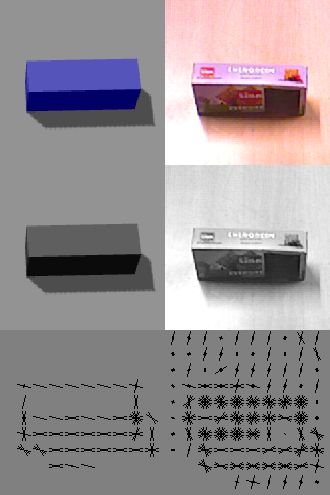
\includegraphics[width=0.74\textwidth]{simulation_vs_real_world_base_case.png}
    \caption{\label{fig:simulation_vs_real_world_0}\ang{0}}
  \end{subfigure}
  \begin{subfigure}[b]{0.238\textwidth}
    \centering
    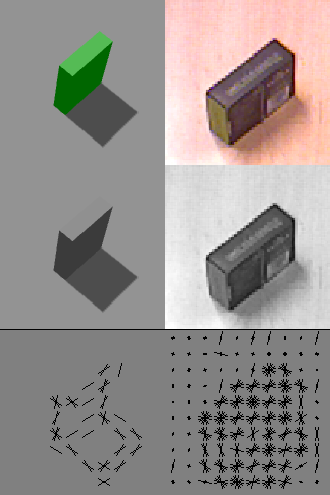
\includegraphics[width=0.74\textwidth]{simulation_vs_real_world_broken.png}
    \caption{\label{fig:simulation_vs_real_world_135}\ang{135}}
  \end{subfigure}
  \caption{\label{fig:pipelines} Processing Pipeline for Real-World vs.
    Environment for Several Angles}
\end{figure}

In both figure \ref{fig:simulation_vs_real_world_0} and figure
\ref{fig:simulation_vs_real_world_135}, the HOG features are far noisier in the
real-world environment than the simulated environment. However, as the
classifier has been trained on these noisy features it can handle the
classification correctly. Additionally, for the simulated box in figure
\ref{fig:simulation_vs_real_world_0} the classifier responds correctly. This is
to be expected given that the shape of the resulting features are almost
characteristic of that angle. However, when considering the simulated box for
figure \ref{fig:simulation_vs_real_world_135}, the classifier classifies
incorrectly. This is evident as after grayscaling the shadow ends up as a very
prominent feature. This distorts the extracted HOG features and causes the
classification to fail. This is less relevant than the real-world performance
but did impact the development process.

With classification handled, the final component was grasping the object. For
the simple boxes that were tested, the grasping was successful in every case.
However, there were limitations to the placement of the object (being too close
or too far) and of the dimensions of the object (too thin). Ultimately, the
resulting system is able to handle the detection, classification, and grasping
of simple box objects robustly. However, more complex configurations involving
multiple overlapping objects or stacked objects cause problems at the angle
classification layer. Further research in segmentation of the objects,
classification of these segments, and the determination of the ordering of
events is required.


% This section should contain:
% \begin{itemize}
% \item A summary of the work.
% \item A thorough explanations of both good and failed experiments.
% \item If there are simulations, a discussion on the differences between simulations and the real world experiments.
% \item A summary of the results.
% \end{itemize}



%%%%%%%%%%%%%%%%%%%%%%%%%%%%%%%%%%%%%%%%%%%%%%%%%%%%%%%%%%%%%%%%%%%%%%%%%%%%%%%%
% \addtolength{\textheight}{-16cm}   % This command serves to balance the column lengths
% on the last page of the document manually. It shortens
% the textheight of the last page by a suitable amount.
% This command does not take effect until the next page
% so it should come on the page before the last. Make
% sure that you do not shorten the textheight too much.



%%%%%%%%%%%%%%%%%%%%%%%%%%%%%%%%%%%%%%%%%%%%%%%%%%%%%%%%%%%%%%%%%%%%%%%%%%%%%%%%

\begin{thebibliography}{99}

\bibitem{Hsu2015} Chih-Wei Hsu and Chih-Jen Lin, A Comparison of Methods for
  Multi-class Support Vector Machines, National Taiwan University, 2015.
\bibitem{Dalal2005} Dalal, N. and Triggs, B., Histograms of Oriented Gradients
  for Human Detection, IEEE Computer Society Conference on Computer Vision and
  Pattern Recognition, 2005, San Diego, CA, USA.
\bibitem{Lowe2004} David G. Lowe, Distinctive Image Features from
  Scale-Invariant Keypoints, University of British Columbia, 2004.
\bibitem{Dong2010} Li Dong, Xinguo Yu, Liyuan Li, and Jerry Kah Eng Hoe, HOG Based
  Multi-Stage Object Detection and Pose Recognition for Service Robot, ICARCV,
  2010, pp. 2495-2500.
\end{thebibliography}

\appendix
\section*{Additional Images}
\begin{figure}[H]
  \centering
  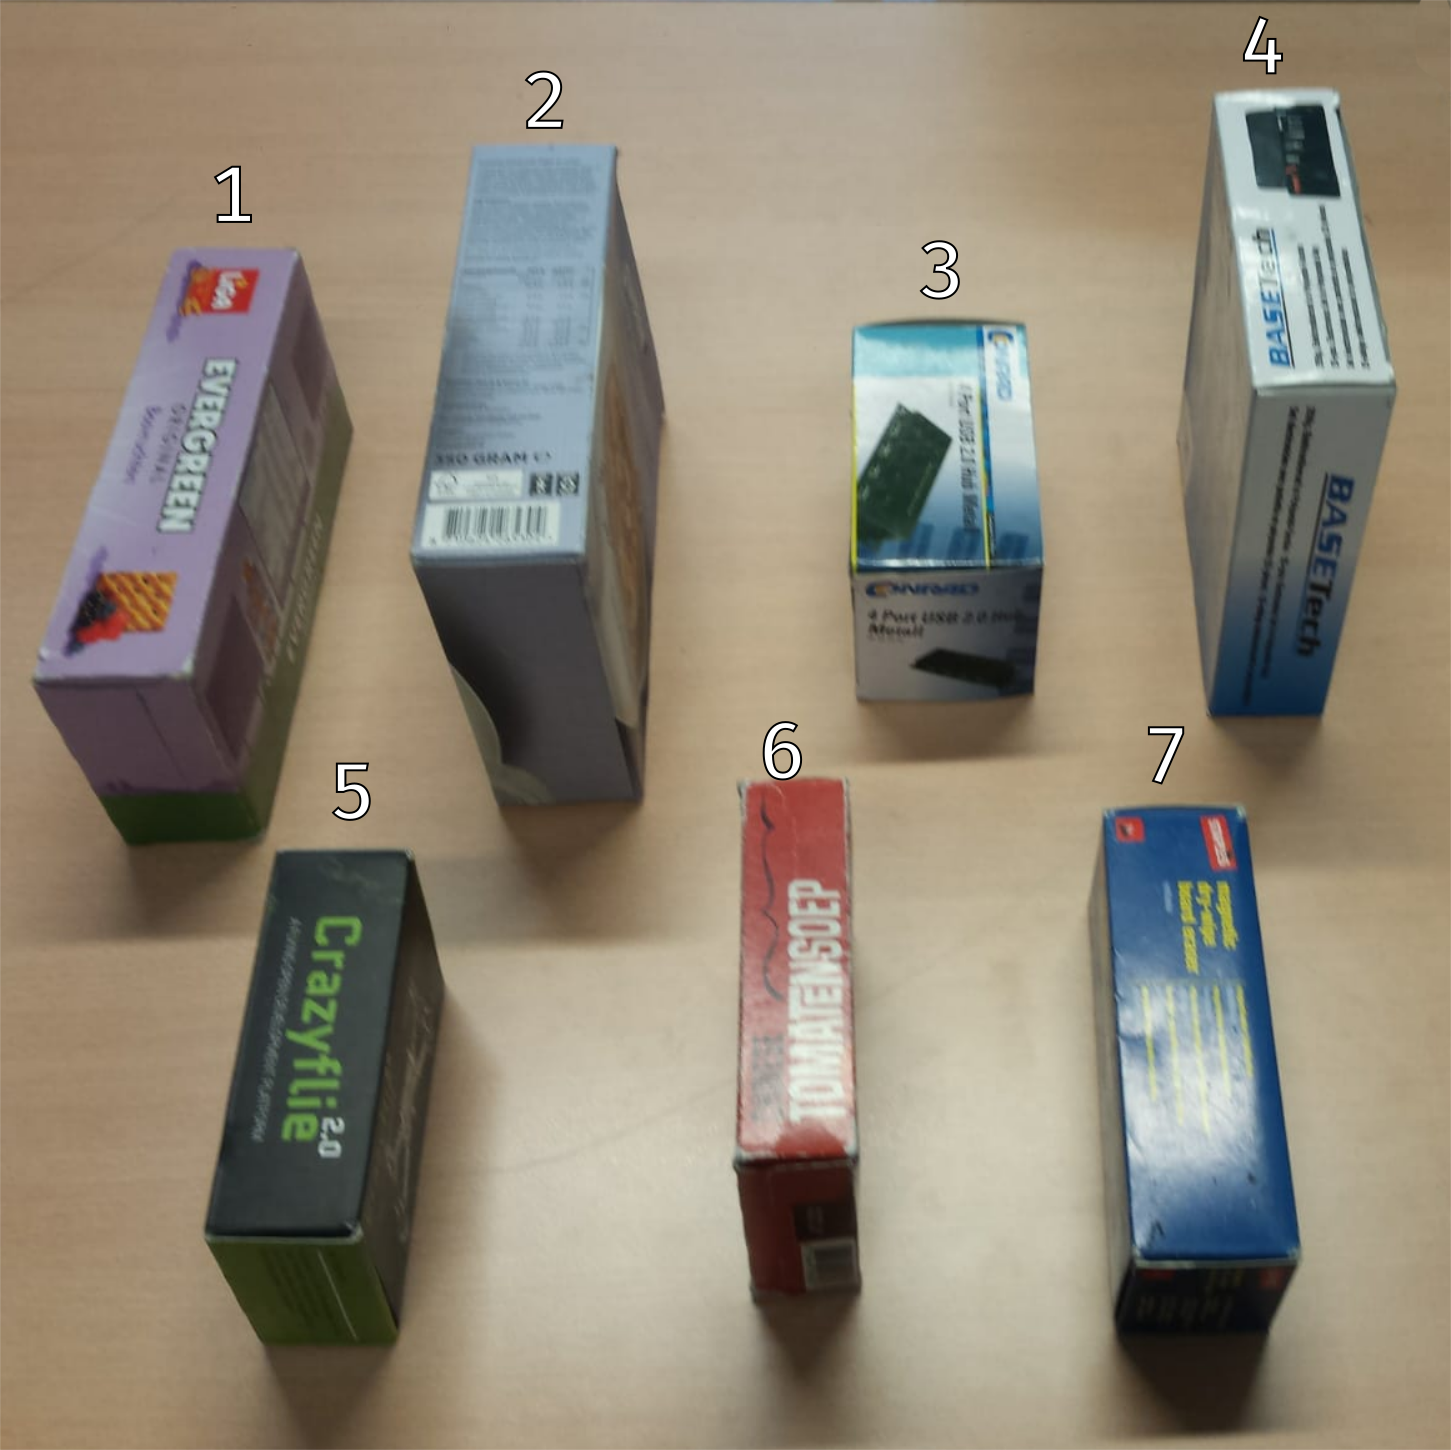
\includegraphics[width=0.9\linewidth]{test_boxes.png}
  \caption{\label{fig:test_boxes} Boxes 1--7 Used for Testing}
\end{figure}


\end{document}